\documentclass{jsarticle}
\usepackage[]{amsmath,amssymb}
\usepackage[]{graphicx}
\usepackage[]{physics}
\usepackage[]{url}
\usepackage[]{hyperref}
\title{行間を読む 猪木慶治・川合光「量子力学I」}
\author{低音}
\date{\today}
\begin{document}

\maketitle
\tableofcontents

\subsection{注意}
誤植・リクエスト等ありましたら、\href{https://note.com/teion_burns/n/nfc8de0fab123}{note}のコメント機能にお願いします。


\subsection*{p. 102 位置演算子の固有関数の具体形}

\subsubsection*{該当箇所}

\textbf{解}  座標演算子$\hat{\bm{r}}$を関数に作用させるには、単にこの関数に$\bm{r}$をかければよいから、
\begin{equation}
    \begin{array}{rcl}\hat{\bm{r}}\psi_{\bm{r}'}(\bm{r})&=&\bm{r}'\psi_{\bm{r}'}(\bm{r})\qquad\textcircled{a}\\\therefore\quad\psi_{\bm{r}'}(\bm{r})&=&C_{\bm{r}'}\delta(\bm{r}-\bm{r}')\qquad\textcircled{b}\end{array}
\end{equation}

\subsubsection*{疑問}
${\therefore}$の間の論理がわからない。

\subsubsection*{解説}

まず位置演算子の定義から
\begin{equation*}
    \hat{\bm{r}}\psi_{\bm{r}_0}(\bm{r})=\bm{r}\psi_{\bm{r}_0}(\bm{r})
\end{equation*}
である。
右辺の$\bm{r}$は二つとも全く同一のものであることに注意。
一方で固有方程式から
\begin{equation*}
    \hat{\bm{r}}\psi_{\bm{r}_0}(\bm{r})=\bm{r}_0\psi_{\bm{r}_0}(\bm{r}).
\end{equation*}
従って
\begin{equation*}
    \bm{r}\psi_{\bm{r}_0}(\bm{r})=\bm{r}_0\psi_{\bm{r}_0}(\bm{r})
\end{equation*}
が全ての$\bm{r}$について成り立っていなければならない。
このためには
\begin{equation*}
    \bm{r}\neq\bm{r}_0\Longrightarrow\psi_{\bm{r}_0}(\bm{r})=0
\end{equation*}
が必要。
ただし、$\psi(\bm{r}_0)$が恒等的に$0$だと物理的に無意味であるから、妥当な関数形としては
\begin{equation*}
    \psi_{\bm{r}_0}(\bm{r})=C_{\bm{r}_0}\delta(\bm{r}-\bm{r}_0)
\end{equation*}
の形を選ばざるを得なくなる。


\subsection*{p. 158 ビリアル定理と物理量ヴィリアル}

\subsubsection*{該当箇所}

\textbf{[解]}  (1) \textcircled{2}の定義より、
\begin{equation*}
    i\hbar\dfrac{d}{dt}\langle\bm{r}\cdot\bm{p}\rangle
    =\cdots
\end{equation*}

\subsubsection*{疑問点}

この解法はどこから出てきたのか。
なぜ位置と運動量の内積を何事もないかのようにスタート地点とするのか。

\subsubsection*{解説}
まず物理量$G:=\displaystyle\sum_i\bm{r}_i\cdot \bm{p}_i$はClausiusが1870年に提唱したもので、ヴィリアル (virial. 語源は羅 vīs「力」)と呼ばれるものであり、ビリアル定理の証明はこの物理量を出発点とする。

導出は\cite{virial wili}所収の古典論におけるビリアル定理の導出と同一手順によって行える。
ヴィリアルの時間微分をとって
\begin{equation}
    \label{eq:dG/dt}
    \begin{array}{rcl}
        \dfrac{dG}{dt}
        &=&
        \displaystyle
        \sum_i(
            \dot{\bm{r}}_i\cdot\bm{p}_i
            +
            \bm{r}_i\cdot\dot{\bm{p}}_i
            )
        \\
        &=&
        \displaystyle
        \sum_i
        \left(
            \dfrac{\bm{p}_i}{m}\cdot\bm{p}_i
            +
            \bm{r}_i\cdot\bm{F}_i
        \right)
        \\
        &=&
        2K
        -
        \displaystyle\sum_i
        \bm{r}_i\cdot\nabla V_i
        .
    \end{array}
\end{equation}
両辺の長時間平均を取ると、左辺は
\begin{equation*}
    \lim_{T\to0} \dfrac{1}{T}\displaystyle\int_0^T\frac{dG}{dt}dt=\frac{G(T)-G(0)}{T}
\end{equation*}
となる。
有限領域内にとどまる運動を考える限り、この右辺の分子は有界であるから、$T\to\infty$の極限で値は$0$となる。
これにより\eqref{eq:dG/dt}右辺の長時間平均は
\begin{equation*}
    \lim_{T\to0}
    \dfrac{1}{T}
    \displaystyle
    \int_0^T
    \left(
        2K
        -
        \sum_i\bm{r}_i\cdot\nabla V_i
    \right)
    dt
    =0
\end{equation*}
となる。
以上によって古典的なビリアル定理が証明される。

テキストの量子力学におけるビリアル定理も、これと全く同じ方針で示している。


\subsection*{p. 163 3次元調和振動子型ポテンシャルのエネルギー固有値とパリティ}

\subsubsection*{該当箇所}

\begin{equation}
    \label{eq:energy eig. val. for 3-dim parity}
    \tag{\textcircled{a}}
    \therefore E_i=\hbar\omega\left(n_i+\dfrac{1}{2}\right), \qquad i=1,2,3 ; n_i=0,1,2,\cdots
\end{equation}
\begin{equation}
    \tag{\textcircled{b}}
    \therefore E=\hbar\omega\left(n+\dfrac{3}{2}\right), \qquad \text{ただし,} n=n_1+n_2+n_3
\end{equation}
パリティは、
\begin{equation}
    \label{eq:parity of 3-dim harm. oscil.}
    \tag{\textcircled{c}}
    P=P_1\cdot P_2\cdot P_3=(-1)^{n_1+n_2+n_3}=(-1)^n
\end{equation}

\subsubsection*{疑問点}

\eqref{eq:energy eig. val. for 3-dim parity}, \eqref{eq:parity of 3-dim harm. oscil.}の式は何を根拠に持ってきたのか。

\subsubsection*{解説}

各成分に対してはp. 74の1次元調和振動子の理論を使うことができ、(3.98)と(3.104)から
\begin{equation*}
    \dfrac{2E}{\hbar\omega}=2n+1
\end{equation*}
である。
これを計算することで\eqref{eq:energy eig. val. for 3-dim parity}を得る。

3次元のパリティを求めるにあたって、まずは1次元調和振動子のパリティを調べる。
1次元調和振動子の波動関数はHermite多項式$H_n$を用いることで、(3.100)を参考に
\begin{equation*}
    \varphi(\xi)
    =
    H_n(\xi)\exp\left(-\dfrac{1}{2}\xi^2\right)
\end{equation*}
となる。
従って$\varphi(-\xi)=\pm\varphi(\xi)$の符号はHermite多項式のパリティによって定まる。
ここでHermite微分方程式の間の漸化式 (導出は\cite{recurrence of Hermite}などに詳しい)
\begin{equation*}
    H_{n+1}(\xi)
    =
    2\xi H_n(\xi)
    -
    2nH_{n-1}(\xi)
\end{equation*}
及び
\begin{equation*}
    H_0(\xi)=1, H_1(\xi)=2\xi
\end{equation*}
から、Hermite多項式$H_n$は$n$が奇数なら奇関数、$n$が偶数なら偶関数であることがわかる。
以上より1次元調和振動子のパリティは$P_{n_i}=(-1)^{n_i}$であることがわかった。

3次元調和振動子の議論に戻る。
3次元でのパリティは
\begin{equation*}
    \begin{array}{rcl}
        \varphi(-\bm{r})
        &=&
        \varphi_1(-x)\varphi_2(-y)\varphi_3(-z)
        \\
        &=&
        (-1)^{n_1}\varphi_1(x)(-1)^{n_2}\varphi_2(y)(-1)^{n_3}\varphi_3(z)
        \\
        &=&
        (-1)^{n_1+n_2+n_3}\varphi(\bm{r})
    \end{array}
\end{equation*}
で表されるので、\eqref{eq:parity of 3-dim harm. oscil.}を得る。


\subsection*{p. 172 ヒルベルト空間のベクトルψを用いたSchrödinger方程式の時間全微分}

\subsubsection*{該当箇所}
(3)' 時間発展は、時間について1階で線形なSchrödinger方程式で表される。
\begin{equation*}
    \tag{6.4}
    i\hbar\dfrac{d}{dt}\psi=\hat{H}\psi
\end{equation*}

\subsubsection*{疑問点}
これまでのSchrödinger方程式は時間偏微分によって
\begin{equation*}
    i\hbar\dfrac{\partial}{\partial t}\psi(\bm{x},t)
    =
    \hat{H}\psi(\bm{x},t)
\end{equation*}
と表してきたが、ここではなぜ左辺に時間全微分$\displaystyle\dfrac{d}{dt}$を使うのか。

\subsubsection*{解説}

まず、ここでの$\psi$はこれまでの波動関数$\psi(\bm{x},t)$のように具体形で表すことができる関数ではなく、より抽象的なもの (Hilbert空間上の状態ベクトル) であることに注意しなければならない。
つまり\textbf{$\bm{x}$を引数とする関数とは仮定していない}。
換言すれば、\textbf{座標系 ($\mathbb{R}^3$など) を定義域とする写像として取り扱っていない}。
同様にして、$t$以外の変数 (例えばテキスト第2章で現れた運動量表示の波動方程式における引数$\bm{p}$) 依存性を仮定していない。

Schrödinger方程式は$\psi$の時間依存性を記述する以上に役割のないものであり、そこに$\bm{x}$など他の変数を入れる意味はない。
故にこの場合、時間全微分と時間偏微分は同一である。

\subsubsection*{補足}
$\bm{x}$を引数とする関数を使って$\psi(t)$を展開できることから位置依存性が生じると思われるかもしれない。
この疑問はブラケットを使うと解決しやすいだろう。
完全性条件を使って$\psi(t)$を$\bm{x}$の関数として展開しようとすると
\begin{equation*}
    \ket{\psi}
    =
    \int d^3x\ket{\bm{x}}\bra{\bm{x}}\ket\psi
    =
    \int d^3x\ket{\bm{x}}\psi(\bm{x})
\end{equation*}
となる。
変数$\bm{x}$は積分のダミー変数であるから、積分外には現れない。
故に$\ket{\psi}$には位置依存性が生じることはない。


\subsection*{p. 208 生成・消滅演算子の交換関係における微分的振る舞い}

\subsubsection*{該当箇所}

また、
\begin{equation*}
    [\hat{a}_i,(\hat{a}_i^\dagger)^{n_i}]=n_i(\hat{a}_i^\dagger)^{n_i-1}
\end{equation*}
は簡単に示せるから、$\cdots$

\subsubsection*{解説}
帰納法で示す。
n_i=1ではテキスト(6.95)を使って$[\hat{a}_i,\hat{a}_i^\dagger]=1$で真。
$[\hat{a}_i,(\hat{a}_i^\dagger)^{n_i}]=n_i(\hat{a}_i^\dagger)^{n_i-1}$が成り立つとき、
\begin{equation*}
    \begin{array}[]{cl}
        &
        [\hat{a}_i,(\hat{a}_i^\dagger)^{n_i+1}]
        \\
        &=
        \hat{a}_i^\dagger[\hat{a}_i,(\hat{a}_i^\dagger)^{n_i}]
        +
        [\hat{a}_i,\hat{a}_i^\dagger](\hat{a}_i^\dagger)^{n_i}
        \\
        &=
        \hat{a}_i^\dagger n(\hat{a}_i^\dagger)^{n_i-1}
        +
        (\hat{a}_i^\dagger)^{n_i}
        \\
        &=
        (n+1)(\hat{a}_i\dagger)^{n_i}
    \end{array}
\end{equation*}
で、$n+1$においても成り立つ。


\subsection*{p. 213 運動量演算子の指数関数の作用}

\subsubsection*{該当箇所}

また、$\hat{p}\ket{q}=i\hbar\dfrac{\partial}{\partial q}\ket{q}$より、一般の$c$に対して、
\begin{equation*}
    \exp(ic\hat{p})\ket{q}
    =
    \exp\left(
        ic\left(
            i\hbar\dfrac{\partial}{\partial q}
        \right)
    \right)
    \ket{q}
    =
    \ket{q-\hbar c}
\end{equation*}
であるが、$\cdots$

\subsubsection*{疑問点}
二つ目の等号。

\subsubsection*{解説}
テキストp. 190 (6.53)とp. 191 (6.58)から
\begin{equation*}
    \ket{a+q}
    =
    \hat{U}(a)\ket{q}
    =
    \exp\left(
        \dfrac{1}{i\hbar}\sum_{i=1}^na_i\hat{p}_i
    \right)
\end{equation*}
であることに注意すると、
\begin{equation*}
    \exp(ic\hat{p})\ket{q}
    =
    \exp\left(
        \dfrac{1}{i\hbar}(-\hbar c\hat{p})
    \right)
    =
    \hat{U}(-\hbar c)\ket{q}
    =
    \ket{q-\hbar c}.
\end{equation*}


\subsection*{p. 230 Penroseのグラフ記法を用いたEuclid群生成子の交換関係の導出}

\subsubsection*{該当箇所}

(ii) 3次元空間のベクトル$\bm{V}$の成分を$V_a\:(a=1,2,3)$のように書くと、$\textcircled{a}$は、
\begin{equation*}
    \hat{R}_a=-\sum_{b, c}\varepsilon_{abc}x_b\dfrac{\partial}{\partial x_c},\quad \hat{T}_a=-\dfrac{\partial}{\partial x_a}
\end{equation*}
と書ける。
少し計算することにより、次の交換子が得られる。
すなわち、
\begin{equation*}
    \tag{7.36}
    \begin{array}{lr}
        \displaystyle
        [\hat{R}_a, \hat{R}_b]
        =
        \sum_{c=1}^3\varepsilon_{abc}\hat{R}_c,
        \\
        \displaystyle
        [\hat{R}_a, \hat{T}_b]
        =
        \sum_{c=1}^3\varepsilon_{abc}\hat{T}_c,
        \\
        [\hat{T}_a, \hat{T}_b]
        =0
        &\blacksquare
    \end{array}
\end{equation*}

\subsubsection*{解説}

Einsteinの縮約もさることながら、Penroseのグラフ記法を使うと便利である。
以下2つを参照してから読まれたい。

\href{ペンローズのグラフ記法によるベクトル解析の公式の表現 | 低音}{https://note.com/teion_burns/n/n5f486f83dd81}

\href{ペンローズのグラフ記法による完全反対称レヒチビタテンソルの公式の表現 | 低音}{https://note.com/teion_burns/n/nb70618989455}

$\hat{R}_a$は図\ref*{fig:Rhat}のように表される。

\begin{figure}
    \centering
    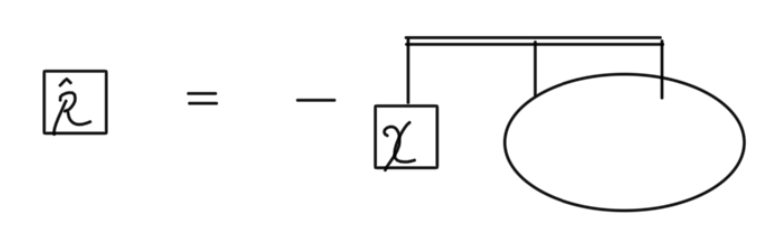
\includegraphics{Rhat.png}
    \caption{Penroseのグラフ記法による$\hat{R}$の表現}
    \label{fig:Rhat}
\end{figure}

これを使って交換子$[\hat{R}_a,\hat{R}_b]$を計算すると、図\ref*{fig:Rhat commutator}のようになる。
ただし、一番右側の上が開いている棒が$a$成分を、下が開いている棒が$b$成分を表すものとする。

\begin{figure}
    \centering
    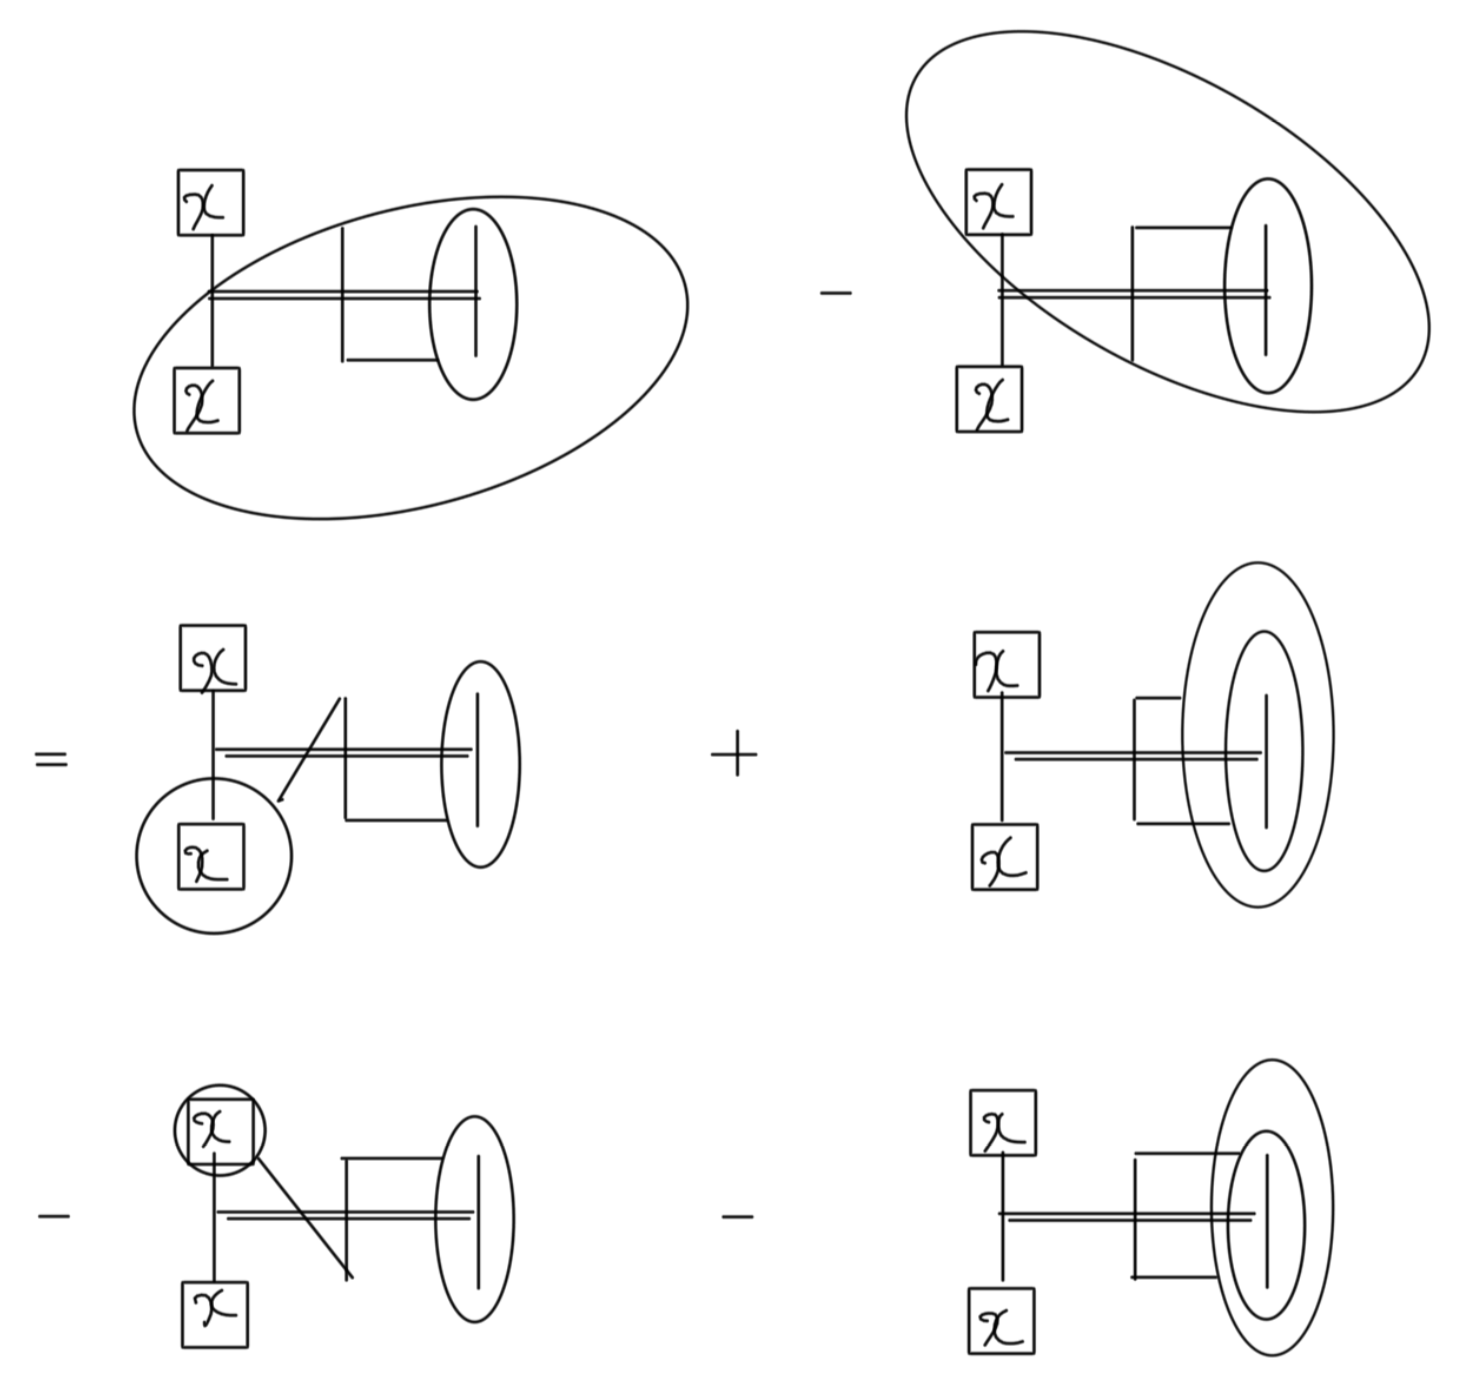
\includegraphics{Rhat-commutator.png}
    \caption{交換子$[\hat{R}_a,\hat{R}_b]$}
    \label{fig:Rhat commutator}
\end{figure}

対称性によって図\ref{fig:Rhat commutator}右下の2つの項が消えて、図\ref*{fig:Rhat symmmetry}の通りになる。

\begin{figure}
    \centering
    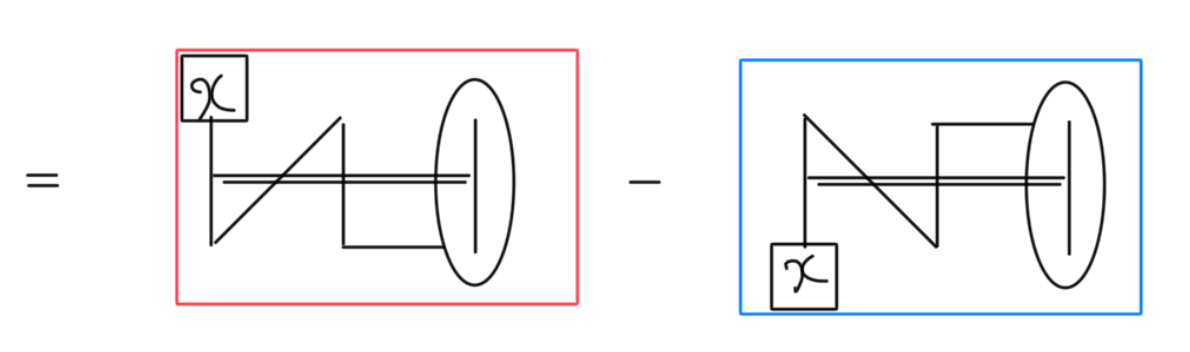
\includegraphics{Rhat-symmmetry.png}
    \caption[]{対称性によって項を消した$\hat{R}$の交換子の表示}
    \label{fig:Rhat symmmetry}
\end{figure}

奇置換するとレビチビタの縮約ができる形になる (図\ref*{fig:Rhat odd replace})。

\begin{figure}
    \centering
    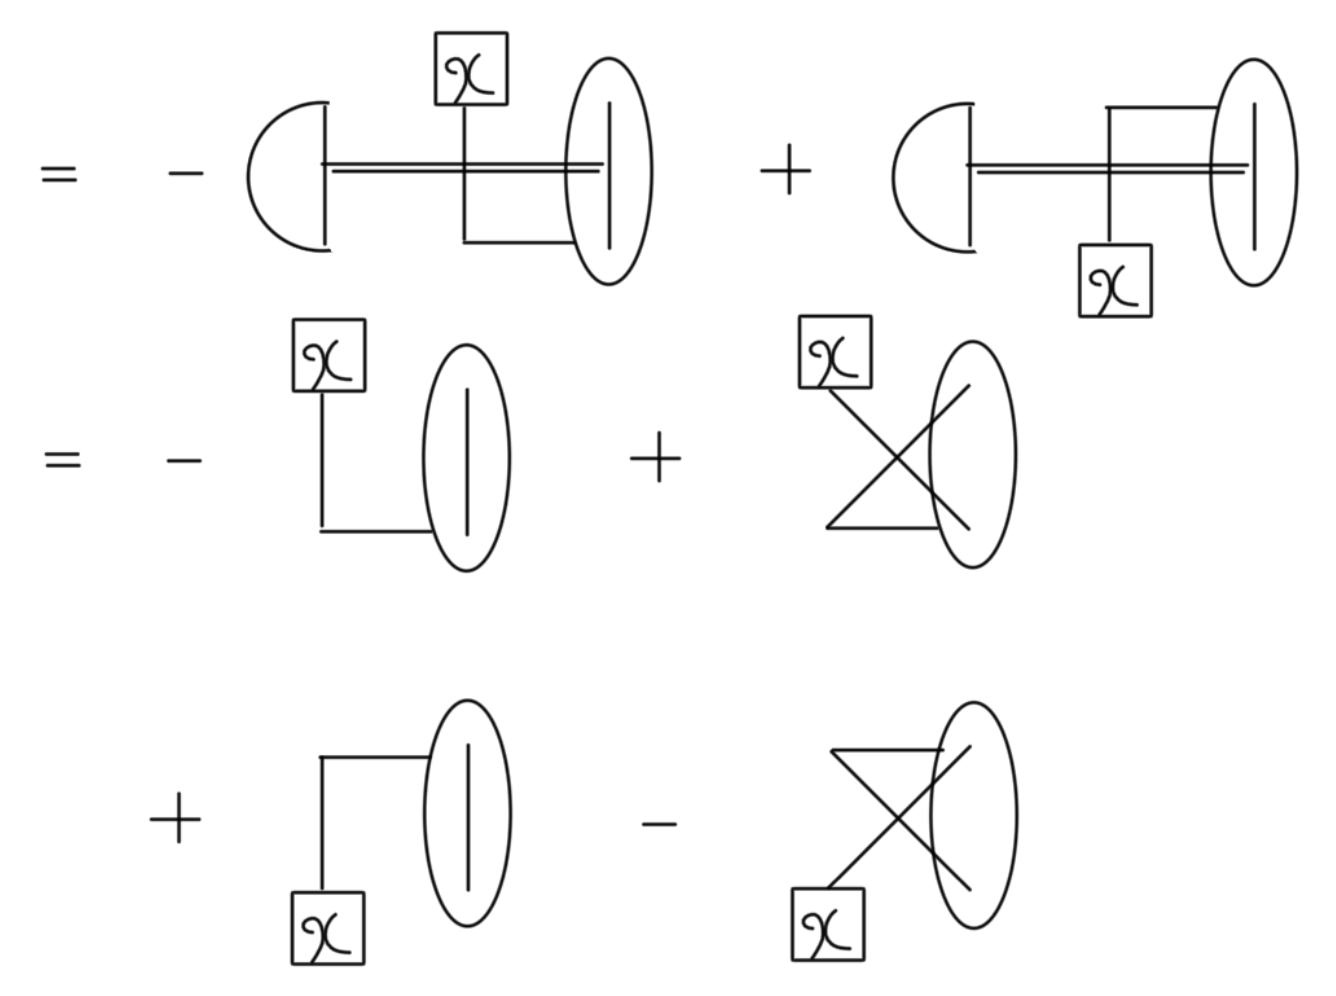
\includegraphics{Rhat-odd-replace.png}
    \caption{レビチビタテンソルの奇置換と縮約}
    \label{fig:Rhat odd replace}
\end{figure}

計算して残るものだけを取り出し、レビチビタの縮約を逆算すると図\ref*{fig:Rhat solution}の通りになる。
ただし、最後は$\hat{R}$の定義を使う。

\begin{figure}
    \centering
    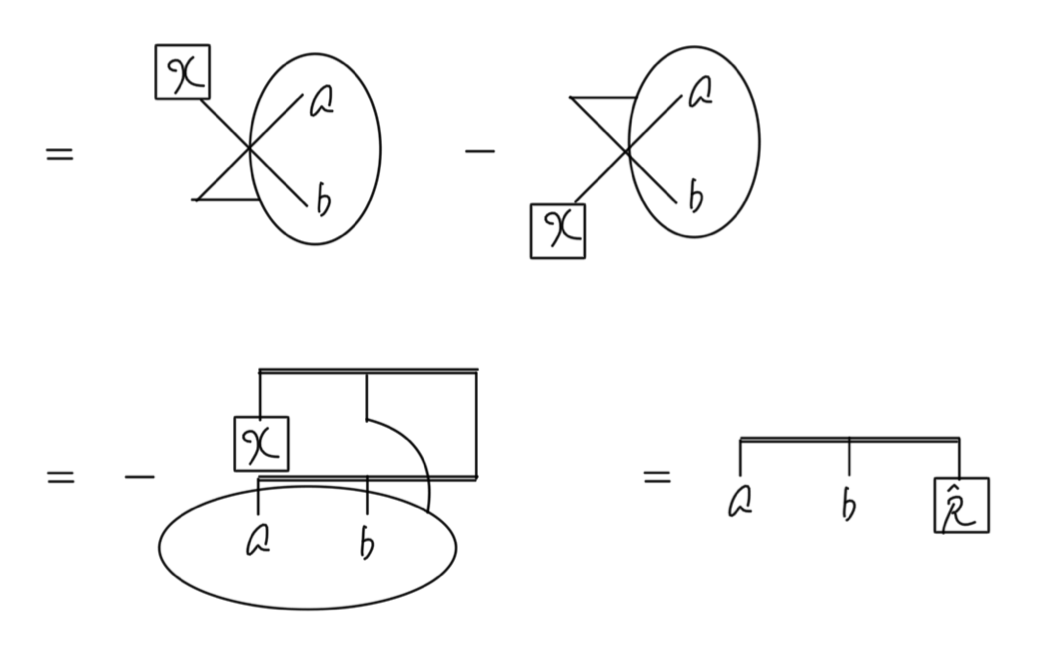
\includegraphics{Rhat-solution.png}
    \caption[]{レビチビタテンソルの逆算で得られる解答}
    \label{fig:Rhat solution}
\end{figure}

他の交換関係は簡単に得られるので割愛する。


\subsection*{p. 281 合流型超幾何微分方程式の極限解析}

\subsubsection*{該当箇所}
1変数$z$の関数$u(z)$に対する微分方程式で、
\begin{equation}
    \tag{A.16}
    \left(
        z\dfrac{d^2}{dz^2}
        +
        (\gamma-z)\dfrac{d}{dz}
        -
        \alpha
    \right)
    u=0
\end{equation}
の形のものを合流形超幾何微分方程式という。
$z$が$0$及び無限大の周りにあるときは、(A.16)は、
\begin{eqnarray}
    \tag{A.17a}
    \left(
        z\dfrac{d^2}{dz^2}
        +
        \gamma\dfrac{d}{dz}
    \right)
    u=0
    \\
    \tag{A.17b}
    \left(
        \dfrac{d^2}{dz^2}
        -
        \dfrac{d}{dz}
    \right)
    u=0
\end{eqnarray}
となるから、1次独立な2つの解は$z\approx0$の周りでは、
\begin{equation}
    \tag{A.18a}
    u\approx z^0, z^{1-\gamma}\quad(z\approx0)
\end{equation}

\subsubsection*{疑問点}
(A.17a)はどんな極限操作によって導出されたのか。

\subsubsection*{解説}

$z$についての次数を考慮すれば良い。
関数$u$をTaylor級数で表して、最低次の項が$z^\beta$であるとする。
$z^\beta$を(A.16)に代入すると、
\begin{equation*}
    \beta(\beta-1)z^{\beta-1}
    +
    \gamma\beta z^{\beta-1}
    -
    \beta z^\beta
    -\alpha z^\beta
    =
    \beta(\beta+\gamma-1)z^{\beta-1}
    +
    o(z^{\beta-1})
    =
    0
\end{equation*}
であり、これを$\beta$について解けば(A.18a)を得る。

ここから遡って考えれば、(A.17a)が(A.16)の中で次数が最低となるものを選んで持ってきていることがわかるだろう。


\begin{thebibliography}
    \bibitem{virial wiki} Wikipedia「ビリアル定理」\url{https://ja.wikipedia.org/wiki/ビリアル定理}
    \bibitem{recurrence of Hermite} 岡山理科大学 若松寛「量子化学ノート」\url{http://www.chem.ous.ac.jp/~waka/compchem/harmonic_oscillator/ho-4-1.html}
\end{thebibliography}
\end{document}
